Operating large-scale clusters is expensive both in terms of
investement to buy all the necessary hardware equipment but also in terms of
human resources that will maintain them. The variety in the jobs
running in a big organization poses a great challenge in the
utilization and efficiency of a cluster. There are long-running
production jobs that should ``never'' stop running, short-living
memory intensive batch jobs that analyze massive amount of data,
testing jobs running with the lowest priority and so forth. At the
same time schedulers should be able to scale to tens of thousands of
nodes per cluster and be highly available with minimum downtime. In order
to tackle these issues there has been a lot research regarding cluster
schedulers or datacenter operating systems as they are also
refered. In this section I will present three different architectures
identified in the current literature based on the taxonomy published
in the Omega paper \cite{41684}. An overview of these architectures is
depicted in Figure \ref{fig:sch_tax}.

\begin{figure}
\centering
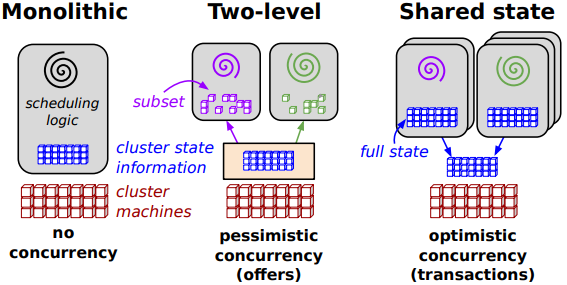
\includegraphics[scale=0.6]{resources/images/Background/schedulers_taxonomy.png}
\label{fig:sch_tax}
\caption{Cluster schedulers architecure \cite{41684}}
\end{figure}

\subsection{Monolithic}
\label{ssec:tax_monolithic}
The first category of schedulers explored is the \emph{monolithic}. In
this architecture there is a single, centralized entity that makes all
the scheduling decisions with no parallelism. A monolithic scheduler
still can facilitate different scheduling policies according to the type
of the workload by providing multiple code paths. Depending on the
type of the job, the execution flow can take different path --
policy. Although, it is tempting to support multiple
scheduling policies, ``it is surprisingly difficult to support a wide
range of policies in a sustainable manner using a single-algorithm
implementation'' \cite{41684}.

Another drawback of monolithic schedulers is the head-of-line
blocking. A small and easy to schedule job might get stack behind a
big and demanding job. This will delay the execution of the former, a
side effect that is not desirable in the enterprize world. Scalability
is another issue that has to be addressed. Since the scheduler runs on
a single instance it can be the bottleneck if the cluster size is big
enough. On the other hand, a monolithic scheduler has a full view of the
cluster and its available resources. For that reason it can make
optimal decisions on the job placement and achieving high utilization
(until it becomes the bottleneck).

A slight variation of a monolithic scheduler is the static
partitioning of the cluster. Each partition will run its own
monolithic scheduler with a separate policy according to the jobs
type. This approach though leads to fragmentation and to sub-optimal
cluster utilization.

A prominent example of a monolithic scheduler is Apache Hadoop YARN
and Hops-YARN. The key characteristic of Hops-YARN is that the state of the
scheduler is stored in the MySQL Cluster which opens the way for
various architectural experimentations resembling shared state schedulers (see
Section \ref{ssec:tax_shared_state}).

\subsection{Two-level}
\label{ssec:tax_two_level}
Two-level

\subsection{Shared state}
\label{ssec:tax_shared_state}
Shared state